% Created 2018-12-05 Wed 21:15
% Intended LaTeX compiler: pdflatex
\documentclass[11pt]{article}
\usepackage[utf8]{inputenc}
\usepackage[T1]{fontenc}
\usepackage{graphicx}
\usepackage{grffile}
\usepackage{longtable}
\usepackage{wrapfig}
\usepackage{rotating}
\usepackage[normalem]{ulem}
\usepackage{amsmath}
\usepackage{textcomp}
\usepackage{amssymb}
\usepackage{capt-of}
\usepackage{hyperref}
\usepackage{color}
\usepackage{minted}
\usepackage{color}
\usepackage{minted}
\usepackage{parskip}
\usepackage{geometry}
\geometry{left=2.5cm,right=2.5cm,top=2.5cm,bottom=2.5cm}
\author{Daniel Moreno Manzano}
\date{\today}
\title{Summary of the quantumsim paper \cite{O_Brien_2017}}
\hypersetup{
 pdfauthor={Daniel Moreno Manzano},
 pdftitle={Summary of the quantumsim paper \cite{O_Brien_2017}},
 pdfkeywords={},
 pdfsubject={},
 pdfcreator={Emacs 25.1.1 (Org mode 9.1.14)}, 
 pdflang={English}}
\begin{document}

\maketitle


\section{Error model parameters}
\label{sec:org7d44cb6}

\begin{table}[htbp]
\caption{\label{tab:orgaa8f932}
Main error model parameters for simulation}
\centering
\tiny
\begin{tabular}{lccp{7cm}}
\hline
Parameter & Symbol & Value & Explanation and notes\\
\hline
Qubit relaxation time & \(T_1\) & 30 \(\mu s\) & Only affects qubits in the excited state. Consistent set of values: [20 - 100 \(\mu s\)]\\
Qubit dephasing time (white noise) & \(T_{\phi}\) & 60 \(\mu s\) & Consistent set of values would be \(2 T_1\) or \(\infty\) (all white noise dephasing eliminated)\\
Decay time & \(T_2\) & 30 \(\mu s\) & \(\frac{1}{T_2} = \frac{1}{T_{\phi}} + \frac{1}{2 T_1}\)\\
Single-qubit gate time & \(T_{g,1Q}\) & 20 ns & \\
Two-qubit gate time & \(T_{g,2Q}\) & 40 ns & \\
Measurement time & \(\tau_m\) & 300 ns & \\
Depletion time & \(\tau_d\) & 300 ns & ?\\
Fast Measurement time & \(\tau_m^{\text{fast}}\) & 100 ns & \\
Fast Depletion time & \(\tau_d^{\text{fast}}\) & 100 ns & ?\\
Readout infidelity & \(\epsilon_{RO}\) & 5\,(-3) & \\
Physical qubit Fidelity & \(\mathcal{F}_{phys} (t)\) & - & \(\mathcal{F}_{phys} (t) = \frac{1}{6}\left(1 + e^{-\frac{t}{T_1}}\right) + \frac{1}{3}\left(1 + e^{-t\left(\frac{1}{2 T_1} + \frac{1}{T_{\phi}}\right)} \right)\)\\
Physical qubit error rate & \(\epsilon_{phys}\) & - & \(\epsilon_{phys} = - \tau_{circuit} \frac{d \mathcal{F}_{phys} (t)}{dt} \textbar_{t=0}=\frac{\tau_{circuit}}{3 T_1}+\frac{\tau_{circuit}}{3 T_{\phi}}\)\\
In-axis rotation error & \(p_{axis}\) & 1\,(-4) & Decay corresponding to shrinking along the y axis because of the single-qubit gates depolarizing noise\\
In-plane rotation error & \(p_{plane}\) & 5\,(-4) & Decay corresponding to shrinking along the x and z axis because of the single-qubit gates depolarizing noise\\
\hline
\end{tabular}
\end{table}

\section{Error models}
\label{sec:org8808a6b}

In the quantumsim module, all gates are applied in the Pauli transfer matrix representation:

$$(R_{\Lambda})_{ij} = \frac{1}{2} Tr(\sigma_i \Lambda \sigma_j)$$

where \(\sigma_i\) are the Pauli operators: \(\sigma_0 = I\), \(\sigma_1 = X\), \(\sigma_2 = Y\), \(\sigma_3 = Z\)

\subsection{Qubit Idling}
\label{sec:orgf61dee9}

While idling for a time \(t\), a transmon in \(|1\rangle\) or in superposition could relax to \(|0\rangle\) or acquire random quantum phase shifts due to \(1/f\) noise sources (flux noise) or others.
The dephasing effect only appears in a superposition state.

\subsubsection{Amplitude-phase damping model}
\label{sec:org84b4bea}

$$R_{\Lambda_{T_1}} = \begin{bmatrix}
 1 & 0 & 0 & 0 \\
 0 & \sqrt{1 - p_1} & 0 & 0 \\
 0 & 0 & \sqrt{1 - p_1} & 0 \\
 p_1 & 0 & 0 & 1 - p_1 \\
\end{bmatrix}$$


$$R_{\Lambda_{T_{\phi}}} = \begin{bmatrix}
 1 & 0 & 0 & 0 \\
 0 & \sqrt{1 - p_{\phi}} & 0 & 0 \\
 0 & 0 & \sqrt{1 - p_{\phi}} & 0 \\
 0 & 0 & 0 & 1 \\
\end{bmatrix}$$

with \(p_1 = 1 - e^{-\frac{t}{T_1}}\) and \(p_{\phi} = 1 - e^{-\frac{t}{T_{\phi}}}\) that are the probabilities for relaxation and pure dephasing, respectively.

\subsubsection{Qubit idling}
\label{sec:org53495f9}

Idling for a duration \(t\):

$$R_{AP (t)} = R_{\Lambda_{T_1}} R_{\Lambda_{T_{\phi}}}$$

\subsection{Single-qubit \(R_y(\pi /2)\) rotations}
\label{sec:orgd1a880a}

"Single-qubit gates [\ldots{}] errors can mostly be attributed to Markovian noise. [\ldots{}] we thus model these errors as Markovian".

"Single-qubit rotations are modeled by sandwiching an instantaneous Pauli transfer matrix, representing the rotation, with periods of duration \(\frac{\tau_{g,1Q}}{2}\) of amplitude and phase damping.
This allows to model the gate for different \(T_1\) and \(T_{\phi}\) [\ldots{}]
However, [\ldots{}] actual gates are more accurately described when adding a [\ldots{}] depolarizing noise to the instantaneous part.
In the Bloch sphere, this decay corresponds to shrinking toward the origin, with factor  \(1 - p_{axis}\) along the y axis and \(1 - p_{plane}\) along the x- and z-axes":

$$R_{R_y (\pi /2)} = R_{AP (\frac{\tau_{g,1Q}}{2})} R_{R_y (\pi /2)}' R_{dep} R_{AP (\frac{\tau_{g,1Q}}{2})}$$

where

$$R_{dep} = \begin{bmatrix}
 1 & 0 & 0 & 0 \\
 0 & 1 - p_{plane} & 0 & 0 \\
 0 & 0 & 1 - p_{axis} & 0 \\
 0 & 0 & 0 & 1 - p_{plane} \\
\end{bmatrix}$$

and \(R_{R_y (\pi/2)}'\) is the Pauli transfer matrix describing the theoretical \(\pi /2\) rotation along the y axis.

\subsection{CZ gates}
\label{sec:orga244349}

"The C-Z gate is achieved by flux pulsing a transmon into the \(|11\rangle \leftrightarrow |02\rangle\) avoided crossing with another, where the 2 denotes the second-excited state of the fluxed transmon.
Holding the transmons here for \(\tau_{g,2Q}\) causes the probability amplitudes of \(|01\rangle\) and \(|11\rangle\) to acquire phases[\ldots{}]

Our full (but simplistic) model of the CZ gate consists of an instantaneous CZ gate with single-qubit phase error \(\delta_{\phi_{1Q}}\) and two-qubit phase error \(\delta_{\phi_{2Q}} = \frac{\delta_{\phi_{1Q}}}{2}\), sandwiched by idling intervals of duration \(\frac{\tau_{g,2Q}}{2}\)."


\subsection{Measurement}
\label{sec:org9f51ae9}

\begin{figure}[htbp]
\centering
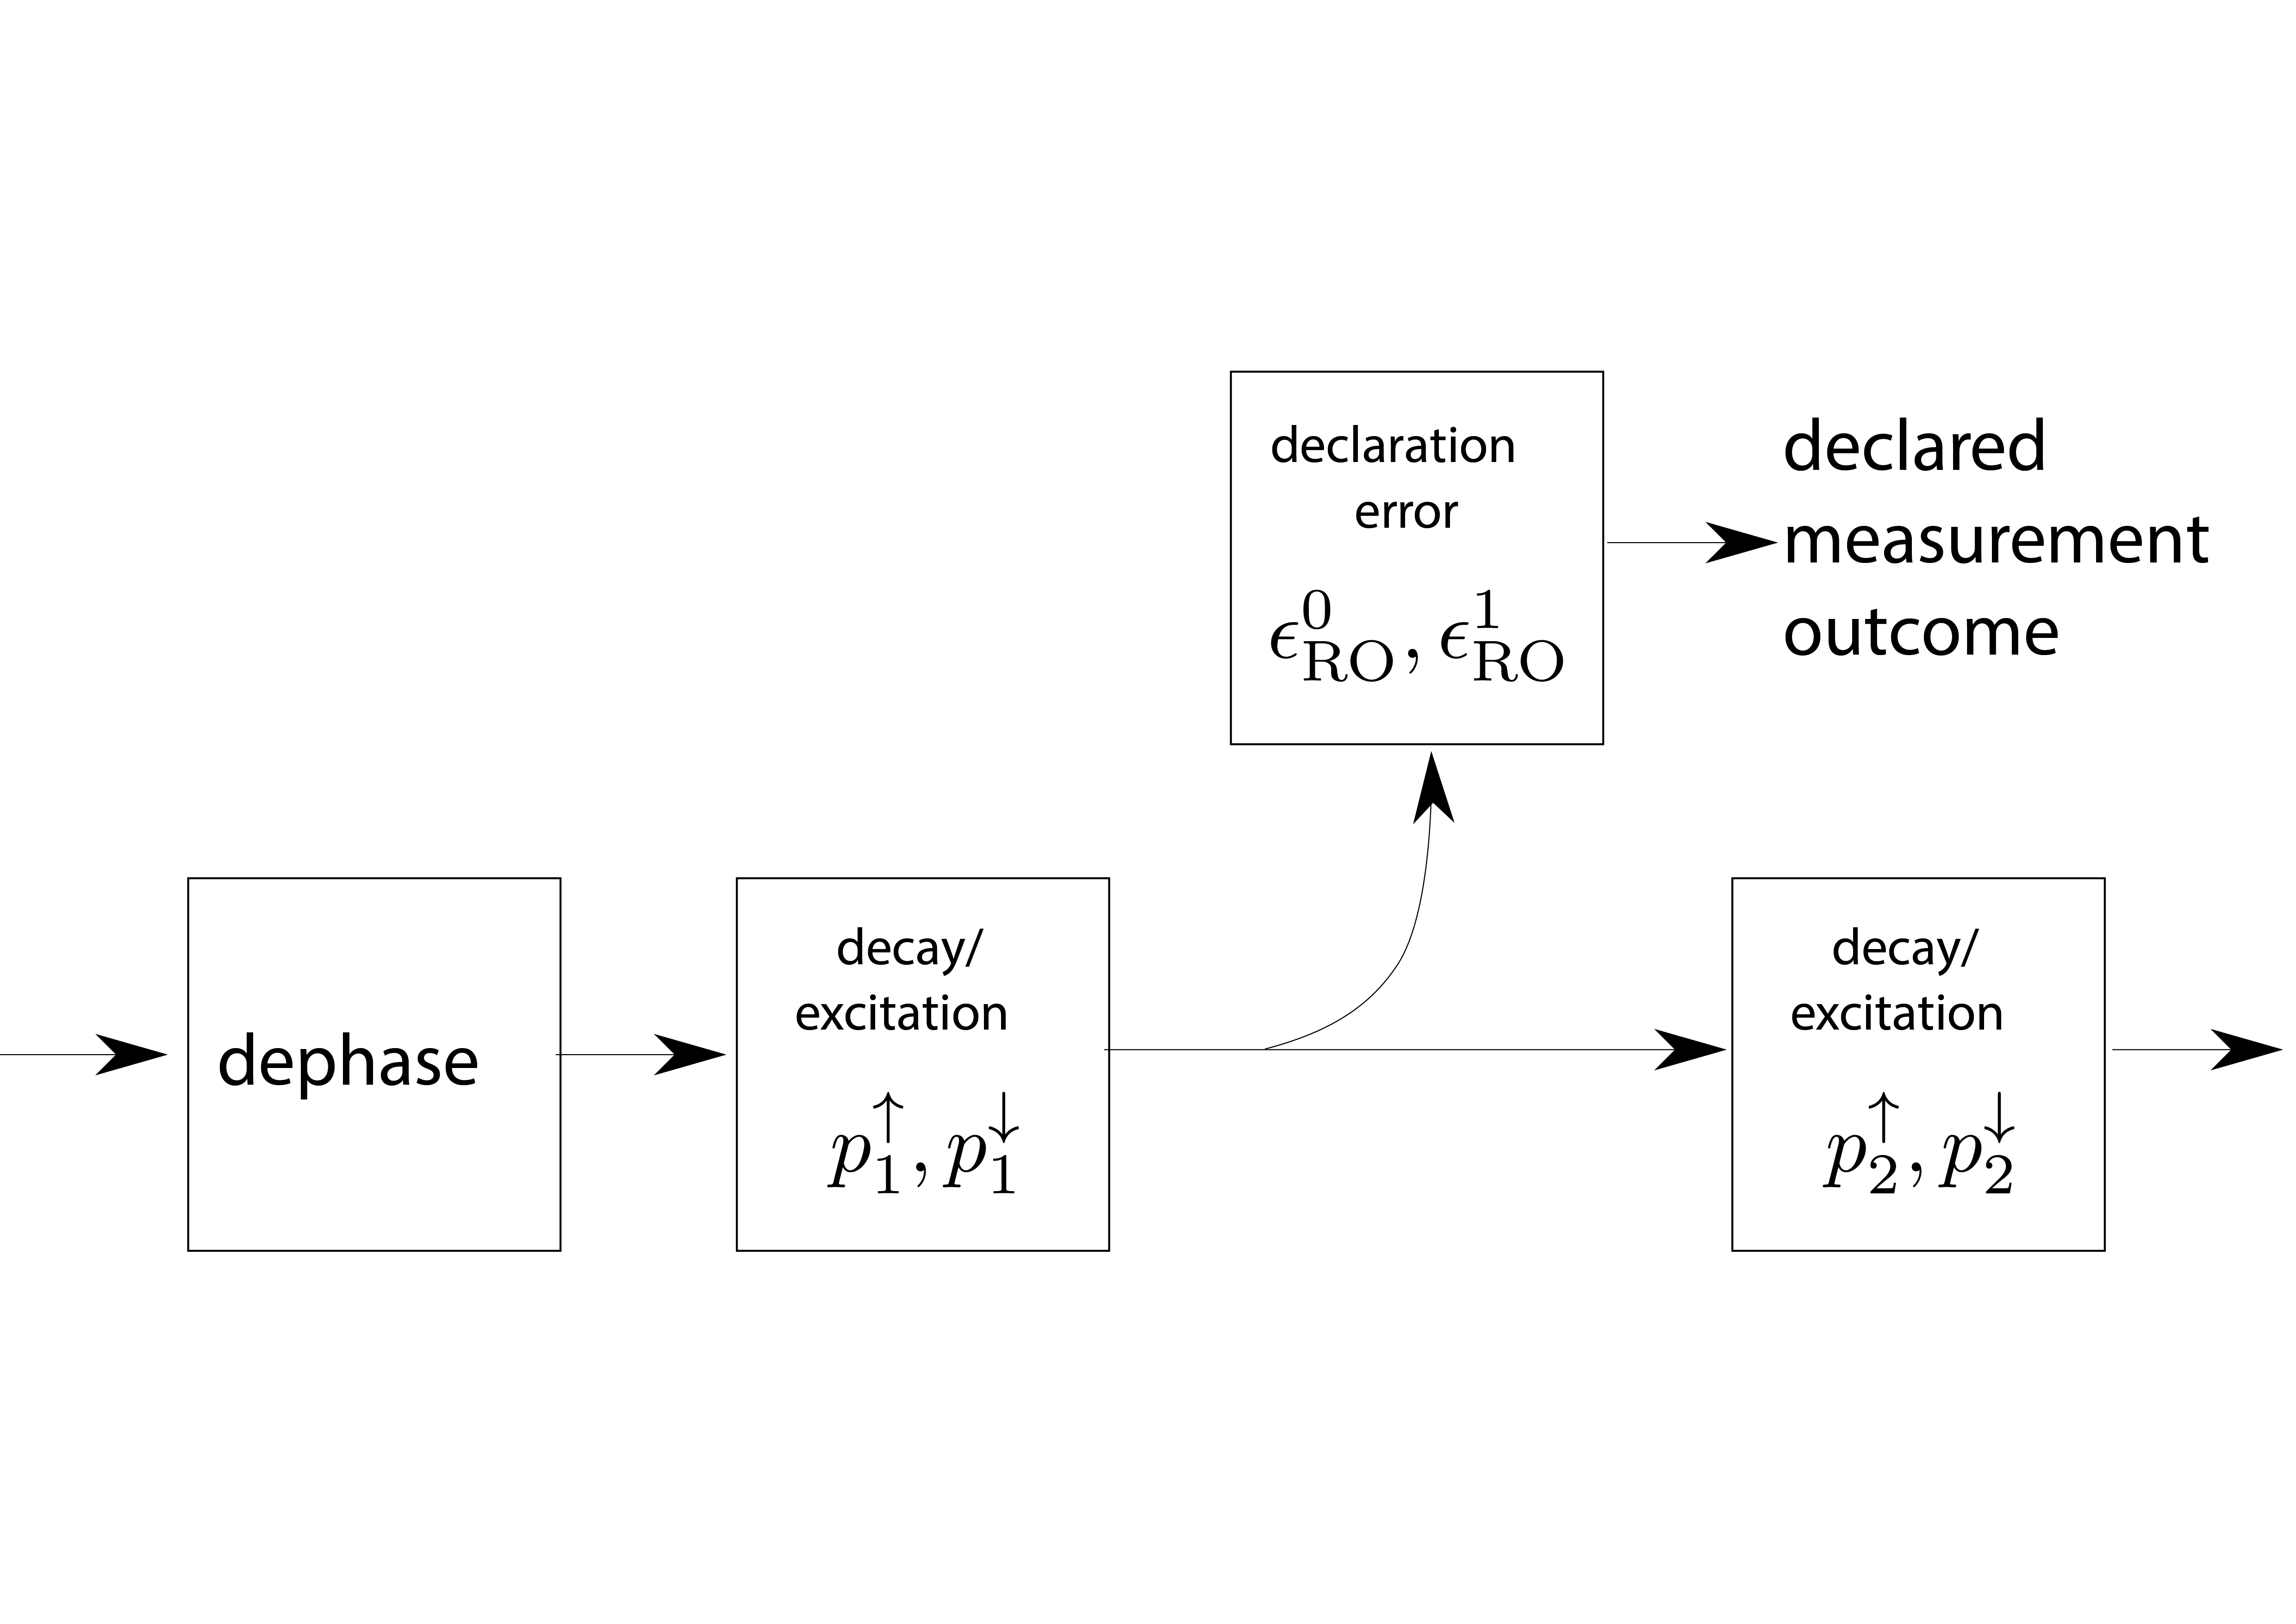
\includegraphics[width=0.5\textwidth]{measure_model.png}
\caption{\label{fig:orgbd6826a}
The model for measurements consists of a dephasing of the qubit followed by a period of decay and excitation with probability \(p_{\uparrow / \downarrow}^{(1)}\). At this point, the qubit state is sampled. The sampling result is subject to a declaration error \(\epsilon_{RO}\), and the qubit state is subject to further decay or excitation with probabilities \(p_{\uparrow / \downarrow}^{(2)}\) before the end of the measurement block}
\end{figure}

The initial dephasing step in the measurement model (Fig. \ref{fig:orgbd6826a}) occurs due to the \hyperref[sec:org1fbd10e]{photon decay} effect.

"We find that the readout errors \(\epsilon_{RO}^{|i\rangle}\) are almost independent of the qubit state \(|i\rangle\), and so we describe them with a single readout error parameter \(\epsilon_{RO}\)".
The outcome-independent declaration error of \(\epsilon_{RO} = \epsilon_{RO}^{1} = \epsilon_{RO}^{0} = 0.15 \%\) is extracted from experiments. 

They ignore effects leading to measurement-induced mixing and non-linearity of the readout resonator, as well as residual photon numbers.

\subsection{Photon decay}
\label{sec:org1fbd10e}
In the presence of photons in a readout resonator, the coupled qubit is affected suffering a \(p_{\phi, photon}\) dephasing.
This dephasing is present whenever the coupled qubit is brought into superposition before the readout resonator has returned to the vacuum state following the last measurement.
This dephasing is then implemented via the same Pauli transfer matrix as \(R_{\Lambda_{T_{\phi}}}\).

\subsection{Flux Noise}
\label{sec:orga1586aa}

During a quantum algorithm, "transmons are repeatedly moved in frequency away from their sweetspot using flux pulses, either to implement a C-Z gate or to avoid one. Away from the sweetspot, transmons become first-order sensitive to flux noise, which causes an additional random phase shift."

"As this noise typically has a \(1/f\) power spectrum, the largest contribution comes from low-frequency components that are essentially static for a single run, but fluctuating between different runs."
"Shifting the transmon from its sweetspot \(f_{q,max}\) to a lower frequency \(f_q (t)\) makes it first-order sensitive to flux noise".

"In our simulation, we approximate the effect of this noise through ensemble averaging, with quasi-static phase error added to a transmon whenever it is flux pulsed."

As one could see in the figures 4 and 5 from the Supplemental information, a little over-rotation  caused by inaccurate calibration of the flux pulse in a single- or two-qubit gate translates in a huge increase of the \(\epsilon_L\).


\section{Effects not taking into account}
\label{sec:org28aa6ab}

They use a simple model for the CZ errors.
They neglect leakage (previous experiments have reduced leakage probability per CZ to \(\approx\) 0.3\%).
Of course this simplification is also in \textbf{quantumsim}.

\section{The quantumsim simulation package}
\label{sec:orgcab828d}

"Quantumsim performs calculations on density matrices utilizing a graphics processing unit in a standard desktop computer [\ldots{}]

One-qubit and two- qubit gates are applied to the density matrix as completely positive, trace preserving maps represented by Pauli transfer matrices. When a gate involving a << new >> qubit must be performed, the density matrix of the system is dynamically enlarged to include that one [\ldots{}]

Qubit measurements are simulated as projective and following the Born rule, with projection probabilities given by the squared overlap of the input state with the measurement basis states. In order to capture empirical measurement errors, we implement a black-box measurement model by sandwiching the measurement between idling processes. After measuring some qubit they remove that qubit from the density matrix.


\section{Observations I find Interesting}
\label{sec:org1b1fbcd}
\subsection{Optimization of logical error rates}
\label{sec:org0e827da}

In Fig. \ref{fig:orgc4585d7} one can see that the optimal time for measuring is 280 ns.

\begin{figure}[htbp]
\centering
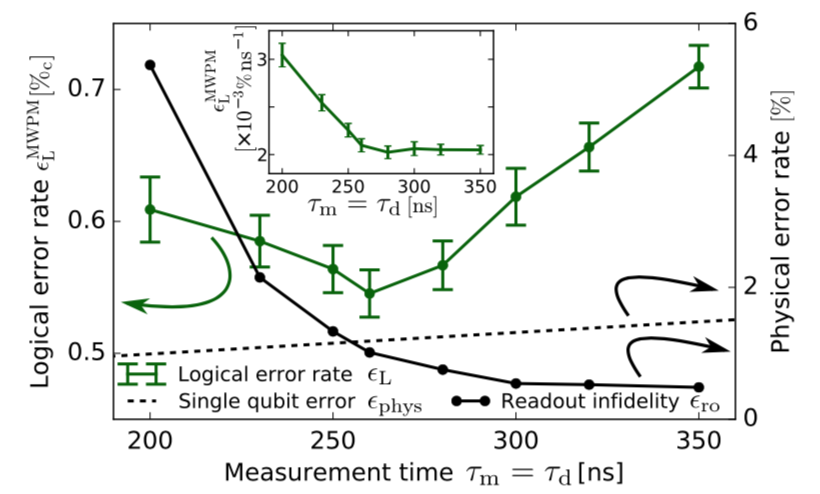
\includegraphics[width=0.7\textwidth]{measure_t_optimization.png}
\caption{\label{fig:orgc4585d7}
Measure time optimization based on the SC-17 logical error rate. Optimal \(\tau_m = 280\) ns}
\end{figure}


\subsection{Projected improvement with advances in quantum hardware}
\label{sec:org1a02258}

\begin{itemize}
\item Memory figure of merit (\(\gamma_m = \frac{\epsilon_{phys}}{\epsilon_{L}}\)). How close are \(\epsilon_{phys}\) and \(\epsilon_{L}\). Metric to check how good the error correction is.

\item Computational performance (\(\gamma_c = \frac{\epsilon_{phys} \tau_{g,1Q}}{\epsilon_L \tau_{cycle}}\)), where, at \(\gamma_c = 1\) the computational break-even point is defined.

\item A value of \(T_1 > 80 \mu s\) for planar transmons is emerging.
\end{itemize}

\subsection{Other observations}
\label{sec:org89b413c}

The following statements are fairly general:

\begin{itemize}
\item "Small quasi-static qubit errors are suppressed by the repeated measurements"
\item If either the ancilla error rate (\(\epsilon_{anc}\)) or the \(\epsilon_{\text{RO}}\) are bigger than \(\epsilon_{phys}\), \(\epsilon_L\) becomes independent of both \(\epsilon_{RO}\) and \(\epsilon_{anc}\)
\item "Optimal cycle parameters for logical error rates per cycle and per unit time are not the same. This implies that logical qubits functioning as quantum memory should be treated differently to those being used for computation"
\end{itemize}



\section{Doubts}
\label{sec:org89eaff0}
\begin{itemize}
\item What is the depletion time?
\item I do not understand the Inset in Fig. \ref{fig:orgc4585d7}
\item What is the difference between qubits used for quantum memory and quantum computation? In our case we consider just computation, isn't it?
\item Surface code is good for Quantum Memory. Which code is good for Quantum Computation?
\item Why do we consider that the measurement time is 300 ns instead of 280 ns, that is the optimum time for logical qubit error rate?
\item Study the optimum times for each gates to minimize the physical qubit error rate
\item At some point \(T_{\phi} = \infty\) is mentioned. Is it possible to clean all the dephasing white-noise.
\item Is the Y rotation gates the only ones affected by the dephasing noise?
\item \sout{What is the flux noise?} \(\to\) "Shifting the transmon from its sweetspot \(f_{q,max}\) to a lower frequency \(f_q (t)\) makes it first-order sensitive to flux noise"
\item What are the quasi-static qubit errors?
\item \sout{Does the \(R_{dep}\) parameter mean that the depolarizing model is included?} \(\to\) I would say so. But only for the single-qubit gates
\item \sout{Is the \(p_{\phi, photon}\) summed to the \(p_{\phi}\) in the \(R_{\Lambda_{T_{\phi}}}\) or how is it done?} \(\to\) is the dephase at the beginning of the measurement model (Fig. \ref{fig:orgbd6826a})
\item What is an adiabatic gate?
\item I do not understand anything in the measurement.
\begin{itemize}
\item What is \(\epsilon_i^{m,o}\), \(a\) and \(b\)
\item Are the ignored effects during measurements important for us? Do not think so.
\end{itemize}
\item Quantumsim is able to work no taking into account the surface code, isn't it?
\item Is this error model the one that they use in quantumsim? Are all the parameters ready or should I look for add some of them?
\item "Ancillas are measured at the end of each cycle, and thus not entangled with the rest of the system". Is this due to the circuit they are using or quantumsim works like that in general
\end{itemize}


\section{Ideas}
\label{sec:org9e11a3a}

\subsection{The physical error rate is related with the depth of a circuit}
\label{sec:org29b8d70}

Considering any quantum circuit, different from the stabilizer circuit from the Surface Code cycle with the next parameters:


\begin{center}
\begin{tabular}{lr}
Depth: & \(d\)\\
Cycle time (minimum operation time): & \(T_{cycle}\)\\
Circuit time: & \(\tau_{circuit} = d \times T_{cycle}\)\\
\end{tabular}
\end{center}

Taking into account the physical error rate function defined in Table 1, we could define the physical qubit error rate of the SC chips for any quantum circuit as:

$$\epsilon_{phys} = \frac{d \times T_{cycle}}{3} \frac{T_{\phi} + T_1}{T_{\phi} T_1}$$

\subsection{Maximum depth given a \(\epsilon_{phys}\)}
\label{sec:org69ebd19}

Given a maximum error rate for the qubits (\(\epsilon_{phys}^{\uparrow}\)) as an upper bound, the maximum depth of the circuit would be:

$$d^{\uparrow} = \frac{3 \epsilon_{phys}^{\uparrow}}{T_{cycle}} \frac{T_{\phi} T_1}{T_{\phi} + T_1}$$

Where any \(d > d^{\uparrow}\) will have a physical error rate bigger than the desired one (\(\epsilon_{phys} > \epsilon_{phys}^{\uparrow}\)).



\bibliography{thesis_plan}
\bibliographystyle{plain}
\end{document}
